%!TEX root = ../../Master.tex
\section{Graph theory}

Graph theory is frequently used in computer science to model some kind of relationship between objects. These objects could be anything. Graph theory is a preferred method to model building complexes, because it can precisely model how e.g. a hallway in a hospital is connected to a room.

In graph theory objects are called \enquote{nodes} or \enquote{vertices}. The two terms can be used interchangeably. In this paper, vertices will describe coordinates or POI (points of interest) in a hospital. Another term in graph theory is an edge. This is basically connecting two vertices and thereby providing a relationship between these vertices. See \cref{fig:labeled_graph}. An edge can be seen as a possible route connecting one coordinate to another. Now in order to describe the relationship between two vertices, we use an weighted graph in which an edge has a number attribute called a weight. A weight can describe the time, distance or any other metric that in some way can describe how two connected vertices are related.\cite{wiki_graph_glos,MIT2012}

We can describe these definitions formally.\cite{MIT2012}
\begin{mydef}
	A graph $G$ is a pair of sets $(V,E)$ where $V$ is a non-empty set of items called vertices or nodes. $E$ is a set of 2-item subsets of $V$ called edges.
\end{mydef}

\begin{figure}[ht!]
    \centering
    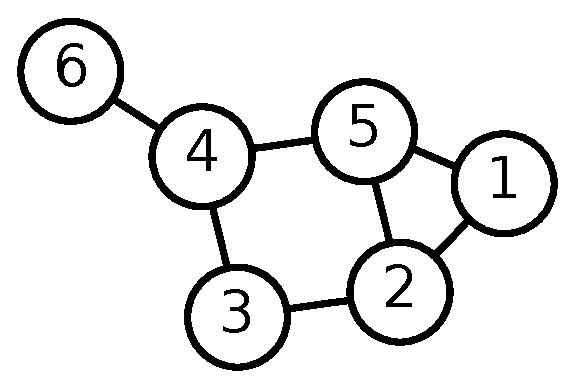
\includegraphics[width=0.5\textwidth]{6n-graf.eps}
    \caption{A labeled simple graph with vertex set $V = \left\{ {1, 2, 3, 4, 5, 6} \right\} $ and edge set $E = \left\{ \left\{ {1,2}\right\}, \left\{ {1,5}\right\}, \left\{ {2,3}\right\}, \left\{ {2,5}\right\}, \left\{ {3,4}\right\}, \left\{ {4,5} \right\} , \left\{ {4,6} \right\} \right\}$. \cite{wiki_graph_glos}}
    \label{fig:labeled_graph}
  \end{figure}

\subsection{Storing a complex as a graph}

\subsubsection{Representing a floor}

Every decision and every change direct is a vertex in our graph, is modelled by vertices connected with edges. Exits, elevators, stair and bridges are vertices for getting from a floor to another, including another building. Vertices that does not classify as one of the previously mentioned are doors, intersection and a change of walking direction. See \cref{fig:Vertices}. Connecting the vertices are edges with a weight, which could be weighted with the distance in meters from one vertex to another.

\begin{figure}[ht!]
    \centering
    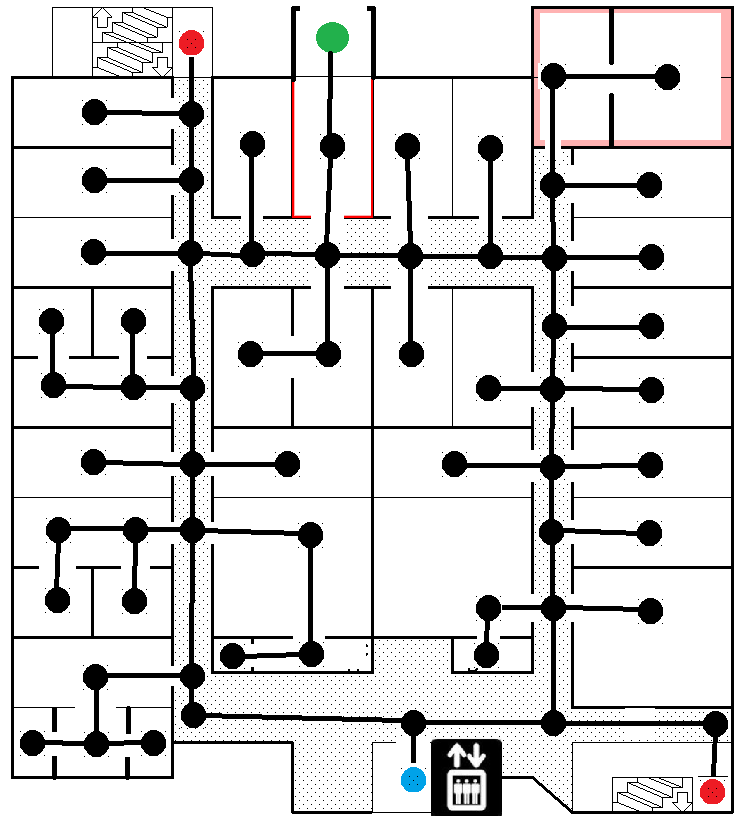
\includegraphics[width=1.5\textwidth]{floorplan_graf}
    \caption{The image Representation how the graph will look like on a Floor Plan for a existing building, the circles are vertices's and lines are edges}
    \label{fig:floorplan_graf}
  \end{figure}
\

\subsubsection{Multiple floors}

A complex such as a hospital usually consist of multiple floors, connected by stairs and elevators as observed at the visit to Sygehus Nord. Representing floors in a graph could be constructed by having edges in between floors. Elevators or stairs are represented by vertices that connects the edges between the floors. Having a graph that models the whole complex can have complications such as overlapping vertices coordinates. Estimating a heuristic value between destination and vertices on two separate floors, means that the heuristic models that does not account for obstacles, would cause the A* algorithm to expand vertices, leading to vertices below the destination on a separate floor than the desired. See \cref{fig:buildingAstar}.

\begin{figure}[ht!]
    \centering
    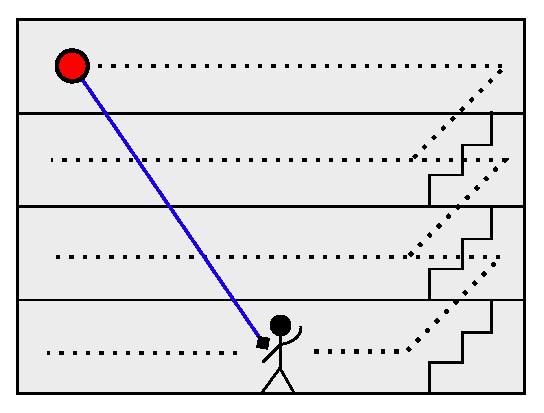
\includegraphics[width=0.5\textwidth]{buildingAstar}
    \caption{How many vertices the A* algorithm would expand, if using the euclidean distance as heuristic}
    \label{fig:buildingAstar}
  \end{figure}

If the complex is divided into separate floor graphs, the algorithm would not have to account for the height coordinates in its heuristic value. A algorithm could evaluate if the source and destination is on the same floor, if not the algorithm could divide the problem into A* searches. First finding a path leading to an elevator or stair which lead the destinations floor. The optimal path from one floor to another can be pre-calculated and stored. 

\subsubsection{Multiple buildings}

The previously described method for modelling floors allows the algorithm to comprehend from complexes of multiple buildings, as seen in \cref{fig:PekhoeS}. The numbers indicate the different floor id's and the letters indicates the connections between the floors. Connection d shows a curved line between 5 and 4 which means they are connected. Every vertex that connects a floor exit with another floor exit, is called a vertex exit\label{e_vertex}. The squares represent a floor.\newline

If we have a building with three floors and one with two floors, the floors will be numbered 1,2,3,4 and 5. The building with the three floors would have its first floor numbered 1, second numbered 2 and last numbered 3. The building with two floors would have its first floor numbered 4 and second floor numbered 5. When modelled, the floors will sorted by their id (number) and stacked as seen on the figure. This means the second floor on two separate buildings will not have the same id. This simplifies a lookup if an individual is on the destination floor height physically, but not in the right building, because a the actual floor height is not relevant as they have been numbered. The thick straight line between 3 and 4, indicates a separation between two buildings. As seen on the figure, there is a exit vertex(a) at floor 1 making a connecting to 2, this could be because of a stair or elevator. The connection(c) between 1 and 4 is possible as both of these floors is at ground level. There is also a connection(b) between 2 and 5 even though the floors is not at ground level or in the same building, this could be they had a bridge leading between them, resulting in a connection. This allows for an exit from one building to another even though the user is not on the first floor. 
\annote{fig 4.4 boer vaere under Multiple buildings og ikke under Pathfinding Algorithms}
\begin{figure}[ht!]
    \centering
    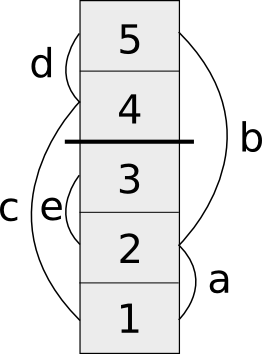
\includegraphics[width=0.5\textwidth]{PekhoeS}
    \caption{Visual representation of floors}
    \label{fig:PekhoeS}
  \end{figure}
